\subsection{Backtracking and Branch-and-Bound}
Backtracking algorithms search the exponential state space of solutions using a depth-first search tree. Within this tree, interior nodes correspond to partial solutions, and leaf nodes correspond to complete solutions. Every node of the tree is labelled,
\begin{enumerate}
	\item Success, if the partial solution can be extended to a \texttt{YES} solution
	\item Failure, if the partial solution cannot be extended to a \texttt{YES} solution
	\item Active, if the partial solution is indeterminate
\end{enumerate}
In the case of a success, the algorithm outputs the solution. In the case of a failure, the algorithm backtracks. In the case of an active label, the algorithm continues searching and pruning the tree.

\begin{marginfigure}
	2-SAT is solvable in polynomial time by the backtracking heuristic, but backtracking can take exponential time to solve an instance of SAT.
\end{marginfigure}

 \begin{defn}[Backtracking]
 	The \textbf{backtracking} procedure is,
 	\begin{algorithm}
	  \caption{Backtracking Procedure}\label{backtracking}
	  \Comment{Start with some problem $P_0$}
	  \Function{Backtrack($P_0$)}{
	  	\Comment{Initialize the set of active problems}
	  	$S \assign \{P_0\}$\;
	  	\While{$S \neq \emptyset$}{
	  		\Comment{Choose a subproblem $P \in S$, expand it into smaller subproblems, and remove $P$ from $S$}
	  		$P \assign P = \{P_1, P_2, \cdots P_k\} \in S$\;
	  		\ForEach{$P_i \in P$}{
	  		\If{$(P_i) = \texttt{Success}$}{
		    	 \Return{$P_i$}\;
		      } \If{$(P_i) = \texttt{Failure}$}{
		      \Comment{Discard $P_i$}
		      $P \assign P - P_i$\;
		      } \Else{
		      \Comment{$P_i$ is indeterminate}
		      $S \assign S + P_i$\;
		      }
	  		}
	  	}
	  }
\end{algorithm}
\end{defn}

The basic approach of backtracking can be extended to optimization problems via the branch-and-bound method. A node is either,
\begin{enumerate}
	\item Infeasible, if there are no feasible completions of a partial solution
	\item Sub-Optimal, if there are feasible completions of the partial solution but they are worse than the optimal solution\footnote{To show that a subtree is sup-optimal, we need a feasible solution to compare it against. Typically, Branch-and-Bound will use Depth-First Search to find an initial feasible solution.}
	\item Feasible, if there are feasible completions to the partial solution and we know the value of the best completion
	\item Active, if the partial solution is indeterminate\footnote{\textbf{Example:} Typically, we branch on the variable that is the most fractional in the linear programming relaxation.}
\end{enumerate}

\begin{defn}[Branch-and-Bound]
	Suppose that we have a minimization problem. Each subproblem will be eliminated if the lower bound on its cost exceeds that of some other solution that we have already encountered. The \textbf{branch-and-bound} procedure is,
 	\begin{algorithm}
	  \caption{Branch-and-Bound Procedure}\label{branchbound}
	  \Comment{Start with some problem $P_0$}
	  \Function{BranchBound($P_0$)}{
	  	\Comment{Initialize the set of active problems}
	  	$S \assign \{P_0\}$\;
	  	\texttt{bestSoFar} $\assign \infty$\;
	  	\While{$S \neq \emptyset$}{
	  		\Comment{Choose a subproblem $P \in S$, expand it into smaller subproblems, and remove $P$ from $S$}
	  		$P \assign P = \{P_1, P_2, \cdots P_k\} \in S$\;
	  		\ForEach{$P_i \in P$}{
	  		\If{$(P_i) = \texttt{Success}$}{
		    	 \Comment{Update best\_so\_far}
		    	 \texttt{bestSoFar} $\assign C(P_i)$\;
		      } \If{$L(P_i) <$ \texttt{bestSoFar}}{
		      \Comment{Lower bound of $P_i$ is less than \texttt{bestSoFar}}
		      $S \assign S + P_i$\;
		      }
	  		}
	  	}
	  }
\end{algorithm}
\end{defn}

We will see an example of the Branch-and-Bound Procedure applied to the Knapsack Problem. First, we will use three facts that were proven in the context of linear programming. These are,

\begin{rmk}
	The inear programming relaxation of an integer programming problem removes the integrality constraint of each variable,
	\begin{multicols}{2}
	$\max \sum_{i=1}^{n} v_{i} \cdot x_{i}$

	s.t. $\sum_{i=1}^{n} w_{i} \cdot x_{i} \leq W$

	$\underbrace{x_{i} \in\{0,1\}}_{x_i \in \mathbb{Z^+}} \quad \forall i \in[n]$

	$\max \sum_{i=1}^{n} v_{i} \cdot x_{i}$

	s.t. $\sum_{i=1}^{n} w_{i} \cdot x_{i} \leq W$

	$\underbrace{0 \leq x_{i} \leq 1}_{x_i \in \mathbb{R^+}} \quad \forall i \in[n]$
	\end{multicols}
\end{rmk}

\begin{cor}
	The feasible region of the relaxed linear program is larger than the feasible region of the original integer linear program\footnote{The feasible region of the linear program allows for fractional solutions.}.
\end{cor}

\begin{cor}
	If the linear program is infeasible, then the integer program is infeasible. Conversely, if the linear program is feasible, then its value is at least as large as the value of the integer program by the previous corollary.
\end{cor}

\begin{ex}{Branch-and-Bound with Knapsack}{label}
	Suppose that a thief has a bag with capacity $W$. There are $n$ items to steal, and each item has an associated value $v_i$ and weight $w_i$. The thief wants to steal the subset of items of \textbf{maximum total value} that fit into the knapsack,
 	\[\begin{array}{ll}
		\operatorname{maximize} & \sum_{i=1}^{n} v_{i} \cdot x_{i} \\
		\text{ subject to } & \sum_{i=1}^{n} w_{i} \cdot x_{i} \leq W \\
		& x_{i} \in\{0,1\} \quad \forall i \in[n]
	\end{array}\]
	We can solve this via exhaustive search using a search tree \texttt{T},
	\begin{center}
		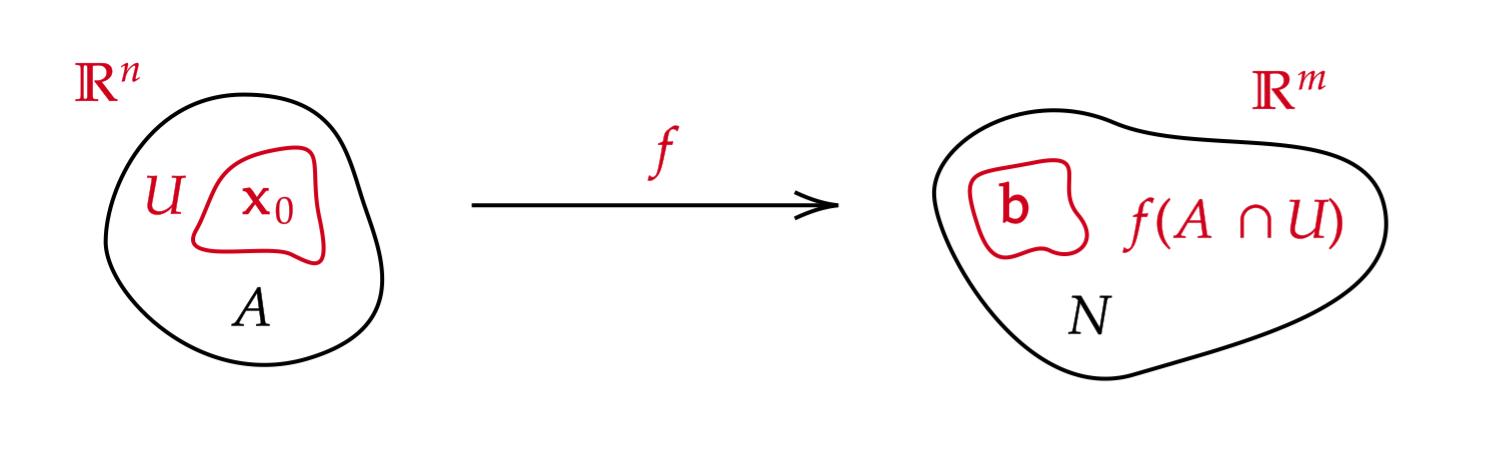
\includegraphics[width=\textwidth]{fig-19.png}
	\end{center}
	but each subtree may be of exponential size to solve. Thus, we require a method for determining if a subtree is either infeasible or worse than the optimal solution. Consider both possibilities for an assignment of \text{$x_1$}. Each decision node in the binary search tree \texttt{T} corresponds to a partial solution,
	\[\left\{x_{1}, x_{2}, x_{3}, x_{4}\right\}=\{0, *, *, *\} \quad\left\{x_{1}, x_{2}, x_{3}, x_{4}\right\}=\{1, *, *, *\}\]

	In particular, at the root of the search tree no variables have been assigned so the corresponding partial solution is empty,
	\[\left\{x_{1}, x_{2}, x_{3}, x_{4}\right\}=\{*, *, *, *\}\]

	This is useful for two reasons,
	\begin{enumerate}
		\item If the partial solution is infeasible, then every completion of the partial solution to a full solution will be infeasible.
		\item If the partial solution leads to low quality solutions, then every completion of the partial solution to a full solution will have a sub-optimal value.
	\end{enumerate}

	We can use \textbf{integer program relaxation} to,
	\begin{enumerate}
		\item Test if every completion of the partial solution is infeasible
		\item Obtain an upper bound on the value of any completion of the partial solution, which bounds the complete solution
	\end{enumerate}
	at the root of every subtree in \texttt{T}.
\end{ex}

\begin{marginfigure}
	\textbf{Solving the Knapsack Problem:}

	\noindent The Knapsack Problem can be solved quickly using a greedy algorithm:
	\begin{enumerate}
		\item Compute the value per weight $V_i := v_i / w_i$ for each item
		\item Determine the object with the maximum ratio, $x^* = \argmax_i V_i$
		\item Assign the knapsack as much of the item $x^*$ as the weight $W$ allows
		\item If the knapsack is not full, recurse on the remaining objects 
	\end{enumerate}
\end{marginfigure}

\begin{ex}{Bad Estimators with Maximum Independent Set}{label}
	Linear programs may lead to bad estimators for integer solutions. Consider the problem of finding the maximum size of an independent set on the graph $K_5$,
	\begin{center}
		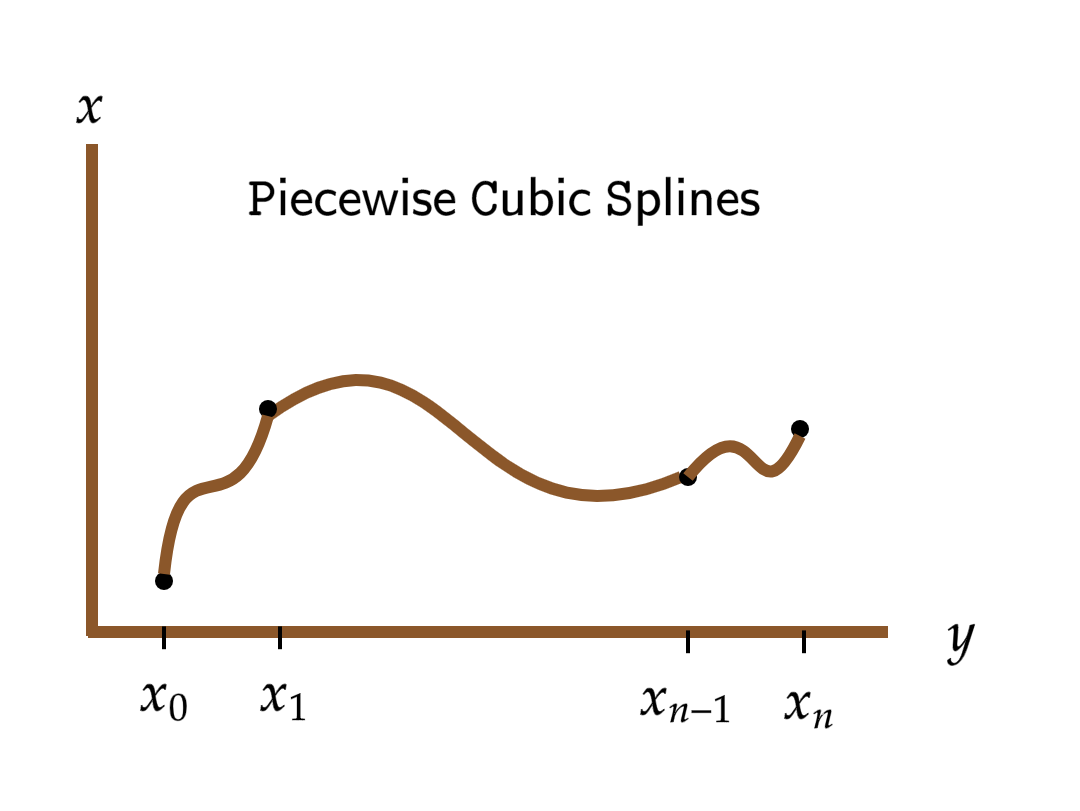
\includegraphics[width=\textwidth]{fig-20.png}
	\end{center}
	\noindent The optimal value of the linear program is $\frac{|V(G)|}{2}$, while the optimal value of the integer program is $1$. This becomes increasingly inaccurate as $|V(G)|$ grows.
\end{ex}

\noindent One possible solution is to use combinatorial estimators\footnote{See Dasgupta, Chapter 9 (p. 273)}.

\begin{ex}{Combinatorial Estimators with Salesman}{label}
	Suppose that we are given a graph \text{$G = (V, E)$} with non-negative edge costs \text{$c_e$}. The goal is to design a tour \text{$T$} that starts and ends at \text{$A$}, includes all other vertices exactly once, and has minimum total cost \text{$c(T) = \sum_e c_e$}. A partial solution \text{$Q$} is a simple path \text{$P$} with endpoints \text{$a$} and \text{$b$} passing through \text{$S \subseteq V \cup \{a,b\}$}. The corresponding subproblem is to find the best completion of the tour, that is, the cheapest complementary path from \text{$b$} to \text{$a$} with intermediate nodes \text{$V - S$}.
	\begin{center}
		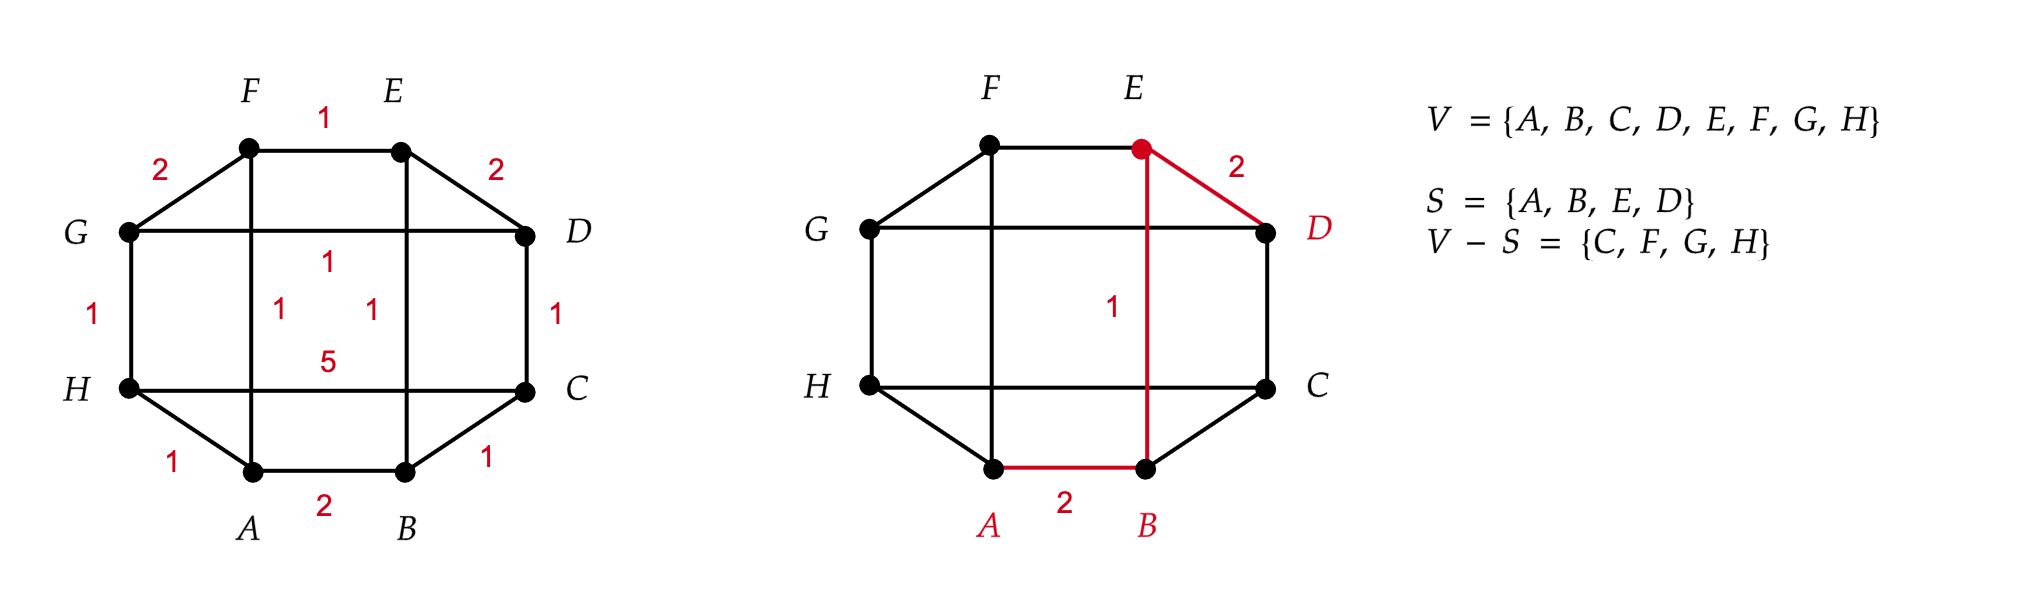
\includegraphics[width=\textwidth]{fig-21.png}
	\end{center}
	The cost of a completion is at least the sum of,
	\begin{enumerate}
		\item The lightest edge from \text{$a$} to \text{$V - S$}
		\item The lightest edge from \text{$b$} to \text{$V - S$}
		\item The minimum spanning tree of \text{$V - S$}
	\end{enumerate}
\end{ex}

\subsection{Local Search}
\begin{defn}[Local Search]
	\textbf{Local search} attempts to find a solution $S^*$ to a problem by making local improvements to the current solution $S$.
	\begin{algorithm}
	  \caption{Local Search (Minimization)}\label{localsearch}
	  \Comment{Start with some initial solution $s$}
	  \Function{LocalSearch($s$)}{
	  	\Comment{Search the neighborhood $\Gamma$ of $s$ for an alternate solution $s^{\prime}$ with a lower cost}
	  	\While{$\exists s^{\prime} \in \Gamma(s)$}{
	  		\If{$cost(s^{\prime}) < cost(s)$}{
	  			$s \assign s^{\prime}$\;
	  		}
	  	}
	  }
\end{algorithm}
\end{defn}

\begin{thm}
	Local search produces a locally optimal solution. 
\end{thm}

\begin{proof}
	We cannot return to a solution that was found previously.
\end{proof}

The neighborhood structure is imposed upon the problem, and it is a central design decision in local search. For example, an algorithm based on Local Search will run quickly with a small neighborhood. Conversely, bigger neighborhoods enable us to find a better solution.

\begin{ex}{Local Search with Maximum Cut}{label}
	In the \textbf{Maximum Cut Problem}, we are given an undirected graph \text{$G = (V, E)$} and a weight \text{$w(e)$} on each edge. We want to separate \text{$V(G)$} into two sets \text{$S$} and \text{$V - S$} so that the total weight of the edges between the two sets is as large as possible. A local improvement is a move of one vertex that produces an increase in the weight of the cut.
	\begin{align*}
		&\text{Let $\mathcal{L}=\varnothing$ and $\mathcal{R}=\mathrm{V}$} \\
		&\text{Repeat:} \\
		&\quad \text{If $\exists v \in V$ such that $\operatorname{cap}(\mathcal{L} \cup v)>\operatorname{cap}(\mathcal{L}):$} \\
		&\quad\quad \text{Set $\mathcal{L} \longleftarrow \mathcal{L} \cup v$} \\
		&\text{Else, If $\exists v \in V$ such that $\operatorname{cap}(\mathcal{L} \backslash v)>\operatorname{cap}(\mathcal{L}):$}\\
		&\quad\quad\text{Set $\mathcal{L} \leftarrow \mathcal{L} \backslash v$}
	\end{align*}

	\begin{thm}
		Any local maximum cut $\delta(\mathcal{L})$ has capacity at least half the capacity of the global maximum cut $\delta(\mathcal{L^*})$.
	\end{thm}

	\begin{proof}
		Let $\delta(\mathcal{L})$ be a local maximum cut, and let $\delta(\mathcal{L^*})$ be the global maximum cut. For any vertex $v$, let $E_v$ be the set of vertices incident to $v$. There are no local improvements for $\mathcal{L}$,
		\[\sum_{e \in E_{v} \cap \delta(\mathcal{L})} u_{e} \geq \sum_{e \in E_{v} \cap \delta(\mathcal{L})^c} u_{e}\]
		In particular, what this means is,
		\[\sum_{e \in E_{v} \cap \delta(\mathcal{L})} u_{e} \geq \frac{1}{2} \cdot \sum_{e \in E_{v}} u_{e}\]
		Therefore,
		\begin{align*}
			\operatorname{cap}(\mathcal{L})&=\frac{1}{2} \cdot \sum_{v \in V} \quad \sum_{e \in E_{v} \cap \delta(\mathcal{L})} u_{e} \\
			&\geq \frac{1}{4} \cdot \sum_{v \in V} \quad \sum_{e \in E_{v}} u_{e} \text{ plugging in the inequality} \\
			&\geq \frac{1}{2} \cdot \operatorname{cap}(\mathcal{L})
		\end{align*}
	\end{proof}
\end{ex}

\begin{marginfigure}
	\textbf{Cut Property of Minimum Spanning Trees:} Assume that edge costs are distinct. If $e$ is the cheapest edge in some cut $\delta(S)$, then $e$ must be in the minimum spanning tree.

	\begin{proof}
		Let $\mathcal{T}^*$ be a minimum spanning tree. Assume that there exists a cut $\delta(S)$ whose cheapest edge $e = (u,v)$ is not in $\mathcal{T}^*$. Since $\mathcal{T}^*$ is a spanning tree, there exists a unique path $P \subseteq \mathcal{T}^*$ from $u$ to $v$. If $\hat{e} \in P$ then $\left(\mathcal{T}^* \backslash \hat{e}\right) \cup e$ is a spanning tree. Moreover, $\hat{e} \in P \cap \delta(S)$ since $|P \cap \delta(S)|$ is odd and consequently $\geq 1$. Swapping $e$ for $\hat{e}$ results in a cheapter spanning tree than $\mathcal{T}^*$.
	\end{proof}
\end{marginfigure}

\begin{ex}{Minimum Spanning Tree Problem}{label}
	The Local Search Algorithm can be used to construct an optimal solution to the \textbf{Minimum Spanning Tree Problem}. We say that a spanning tree $\hat{T}$ is in the neighborhood of a spanning tree $T$ if they differ in exactly one edge,
	\[\Gamma(\mathcal{T})=\{\hat{\mathcal{T}}: \mathcal{T}=(\hat{\mathcal{T}} \cup e) - \hat{e} \text{ where } e \in \mathcal{T} \text{ and } \hat{e} \in \hat{\mathcal{T}}\}\]
	
	We will search for an improving swap that reduces the total cost of the spanning tree.
	\begin{align*}
		&\text{Let $\mathcal{T}$ be a spanning tree.} \\
		&\text{While $\exists \hat{\mathcal{T}} \in \Gamma(\mathcal{T})$ s.t. $c(\mathcal{\hat{T}}) < c(\mathcal{T})$}: \\
		&\quad \text{Set $\hat{\mathcal{T}} \leftarrow \mathcal{T}$}
	\end{align*}
	This outputs a locally minimum spanning tree \text{$\mathcal{T}$}, but we can show that it is in fact the globally minimum spanning tree \text{$\mathcal{T}^*$}. Assume not. If \text{$\mathcal{T} \neq \mathcal{T}^*$}, then \text{$\exists e \in \mathcal{T}^* - \mathcal{T}$}. By the Cut Property, \text{$e$} is the cheapest edge in some cut \text{$\delta(S)$}. Since \text{$\mathcal{T}$} is a spanning tree, there is a unique path $P$ in $\mathcal{T}$ from $u$ to $v$. Thus, there is an edge \text{$\hat{e} \in P \cap \delta(S) \text { with } \hat{e} \neq e$}. But then \text{$\hat{\mathcal{T}}=(\mathcal{T} \cup e) - \hat{e}$} is a cheaper spanning tree than $\mathcal{T}$.
\end{ex}

\begin{ex}{Local Search with Salesman}{label}
	A tour $\hat{\mathcal{T}}$ is said to be in the neighborhood of $\mathcal{T}$ if they differ in exactly two edges. The Local Search Algorithm looks for an improving 2-swap that reduces the cost of the tour. However, there might be an exponential number of iterations needed to solve the Travelling Salesman Problem in this way. Moreover, the final tour is only guaranteed to be locally optimal. 
\end{ex}